\section{Kompression}\label{sec:compression}

\subsection{Motivation}

Unabhängig davon, ob man eine Ausstellung in einem Museum gestaltet oder eine Webseite erstellt, lässt sich fast jede für Besucher oder Benutzer konzipierte Darstellung durch den Einsatz von Bildern aufwerten. Dieses lässt sich durch den Einsatz von 3D-Modellen, mit welchen der Benutzer durch Drehen, Zoomen, etc. interagieren kann, noch deutlich steigern. Abgesehen davon, dass dies in einer Ausstellung nur durch den Einsatz von Rechnern, wie beispielsweise von Tablets, möglich ist, sind damit jedoch einige technische Herausforderungen verbunden.

Einerseits erwartet der Benutzer ein möglichst realistisches Erlebnis, was nur durch hochaufgelöste 3D-Modelle und den damit einhergehenden großen Datenmengen möglich ist. Dennoch soll das Modell möglichst ohne Latenz angezeigt werden und flüssige Interaktion erlauben. Soll die Darstellung darüber hinaus auf einem mobilen Endgerät des Benutzers, wie beispielsweise einem Smartphone, stattfinden, das einerseits nur eingeschränkte Rechenkapazität bietet und auf das andererseits die gesamten Daten für jeden Benutzer separat übertragen werden müssen, entsteht hier ein Gegensatz, für den ein geeigneter Kompromis zu finden ist.

Dieser Kompromis besteht darin, die 3D"=Modelle nicht in der höchsten verfügbaren Auflösung dem Benutzer darzustellen, sondern in einer dem Anwendungsfall und dem Endgerät angemessenen Größe. Beispielsweise ist für eine ansprechende Anzeige auf einem Smartphone"=Bildschirm eine geringere Auflösung notwendig als auf der Workstation eines Museumsmitarbeiters mit entsprechend großem Bildschirm, die auch dementsprechend leistungsfähig ist, und über welche dieser Mitarbeiter das angezeigte Objekt erforschen möchte. Aus diesem Grund ist es sinnvoll, in der Medien-Datenbank die gespeicherten 3D"=Modelle in verschiedenen Auflösungen bereit zu halten, weshalb diese in der Regel beim Hochladen in die Datenbank automatisch komprimiert werden.

Die eben beschriebene Problematik tritt nicht nur bei 3D"=Modellen auf, sondern auch bei herkömmlichen zweidimensionalen Bildern. Da auch solche Medien in der Medien"=Datenbank gespeichert werden sollen, sind auch Bilddateien zu komprimieren, was sich sehr einfach durch das Verringern der Auflösung bewerkstelligen lässt. Von jedem hochgeladenen Bild werden also komprimierte Versionen in verschiedenen Auflösungsstufen erstellt, auf welche anschließend zugegriffen werden kann.

In diesem Kapitel wird nach einer kurzen Erläuterung der theoretischen Grundlagen auf die an die ViSIT"=Medien"=Datenbank angebundene Kompressions"=Komponente und deren Bedienung, die über eine Web-Oberfläche erfolgt, eingegangen. Abschließend wird die Schnittstelle, über welche die Kompressions"=Komponente unabhängig von der dafür verfügbaren Web-Oberfläche oder der ViSIT"=Medien"=Datenbank angesprochen werden kann, spezifiziert.

\subsection{Grundlagen}

Bei 3D-Modellen gilt es grundsätzlich zwischen der Geometrie, durch welche die Form der Oberfläche eines Objekts beschrieben wird, und der Textur, durch welche die Färbung der Oberfläche ausgedrückt wird, zu unterscheiden. Während die Geometrie obligatorisch für ein 3D-Modell ist, muss nicht zwangsläufig eine Textur existieren. Nicht jedes Digitalisierungsverfahren ist in der Lage, Texturdaten zu erfassen, wie beispielsweise ein Laserscanner. Im Folgenden werden Aufbau und Kompression dieser beiden Bestandteile eines 3D-Modells behandelt.

\subsubsection{Geometrie von 3D-Modellen}

Herkömmliche 3D"=Modelle, die ausschließlich die Oberfläche eines Objekts und nicht dessen Inneres beschreiben, bestehen aus mehreren Punkten im dreidimensionalen Raum, die \emph{Vertices} genannt werden. Diese Punkte werden zu Flächen, den sogenannten \emph{Faces} verbunden, wobei es sich hier in vielen Fällen um Dreiecke handelt. Die Anzahl der Ecken eines Faces wird als dessen \emph{Ordnung} bezeichnet. Die Kanten dieser Flächen, die Verbindungen zwischen zwei Vertices darstellen, werden \emph{Edges} genannt. Die Gesamtheit aller Vertices und Faces eines 3D"=Modells wird auch als \emph{Mesh} bezeichnet. Die soeben genannten Begriffe werden in Abbildung \ref{schlenke:fig:fundamentals:geo} grafisch dargestellt.

\begin{figure}
\centering
\subfloat[Vertex]{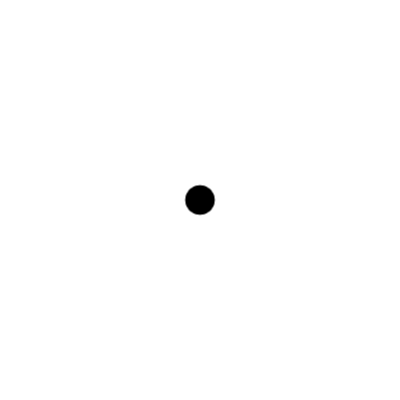
\includegraphics[width=0.25\textwidth]{Figures/schlenker/fundamentals/basicVertex.png}}
\qquad
\subfloat[Edge]{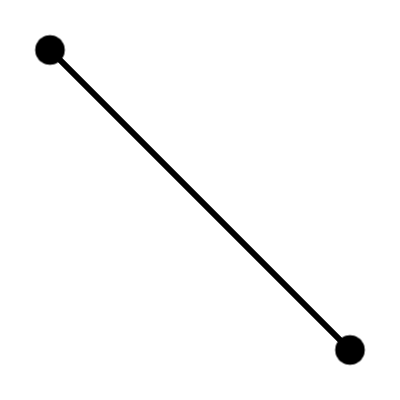
\includegraphics[width=0.25\textwidth]{Figures/schlenker/fundamentals/basicEdge.png}}
\qquad
\subfloat[Face]{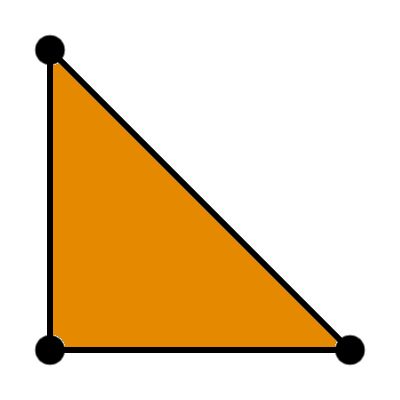
\includegraphics[width=0.25\textwidth]{Figures/schlenker/fundamentals/basicFace.png}}\\
\subfloat[Mesh]{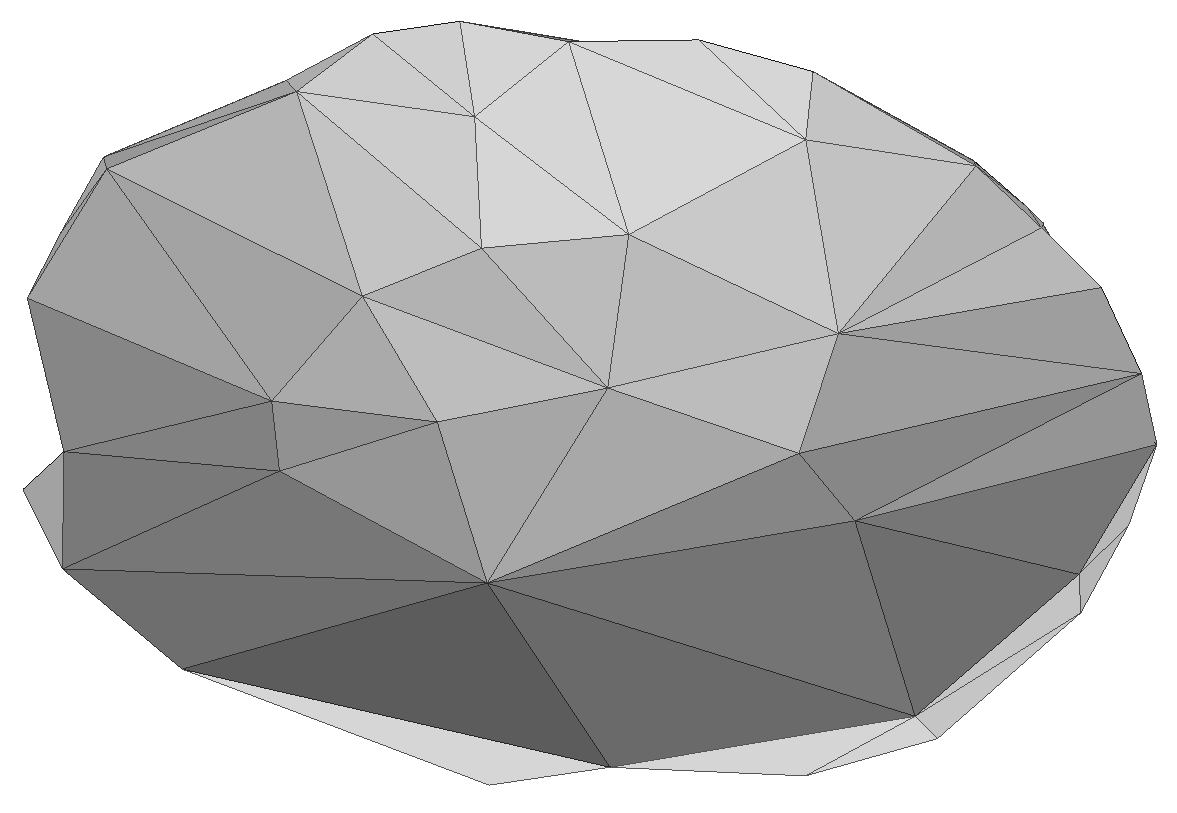
\includegraphics[width=0.70\textwidth]{Figures/schlenker/fundamentals/basicMesh.png}}
\caption{Grundlegende Elemente der Geometrie eines 3D-Modells}
\label{schlenke:fig:fundamentals:geo}
\end{figure}

Während bei einfachen Dateiformaten, wie beispielsweise dem STL-Format\footnote{\url{http://www.fabbers.com/tech/STL_Format}}, für jedes Face die Koordinaten eines jeden Eckpunkts separat gespeichert werden, wird die dadurch verursachte Redundanz zum Beispiel bei OBJ-Dateien\footnote{\url{http://www.martinreddy.net/gfx/3d/OBJ.spec}} vermieden, indem zunächst alle Vertices in Form der Koordinaten einmalig angegeben werden und anschließend bei der Definition der Faces auf diese Vertexdefinition indexbasiert zugegriffen wird.

Bei Meshes, die ein reales Objekt beschreiben, sollte dieser möglichst einer orientierbaren stetigen zweidimensionalen Mannigfaltigkeit, die in den dreidimensionalen Raum eingebettet ist, entsprechen \cite[S.~3]{botsch2010}. Dies hat zur Folge, dass für jeden Punkt im Raum eindeutig entschieden werden kann, ob er im Inneren oder im Äußeren des Objekts liegt. Dies impliziert beispielsweise, dass kein Edge Teil von mehr als zwei Faces sein kann. Jedoch sind auch an die Vertices bestimmte Bedingungen zu stellen, wobei für Details auf \cite[S.~11f]{botsch2010} verwiesen wird.

\subsubsection{Textur von 3D-Modellen}

Die Textur eines 3D"=Modells beschreibt dessen Färbung der Oberfläche, wodurch ihr eine äußerst wichtige Bedeutung für das visuelle Erlebnis beim Betrachten des Modells zukommt. Sie wird in der Regel getrennt von den eigentlichen Geometriedaten in einer separaten Bild"=Datei gespeichert. Für jedes Face wird dann durch die sogenannten \emph{Texturkoordinaten} festgelegt, welcher Ausschnitt des Textur-Bildes auf diesem Dreieck angezeigt wird. Pro Face werden also für jeden Eckpunkt zwei Werte gespeichert, durch welche eine eindeutige Position im Bild definiert wird. Da in der Regel bei den meisten Vertices alle angrenzenden Faces die gleichen Texturkoordinaten verwenden, wird dieses Paar von Werten beispielsweise bei OBJ-Dateien nur einmal gespeichert, worauf anschließend bei der Beschreibung der Faces indexbasiert zugegriffen wird.

Manchem Leser stellt sich hier die Frage, ob generell die Verwendung von einem Paar Texturkoordinaten pro Vertex, welches dann für alle angrenzenden Faces verwendet wird, nicht ausreichend wäre. Hier spielt jedoch die Geometrie des 3D"=Modells, genauer deren \emph{Topologie}, eine wichtige Rolle. Entspricht diese einer (verzerrten) Ebene, so wäre diese Vereinfachung in der Tat ausreichend. Betrachtet man aber beispielsweise eine Kugel, so lässt sich das zweidimensionale Bild nicht über die Kugel legen, ohne dass eine Kante entsteht, an welcher mindestens zwei Ränder des Bildes aneinandergrenzen. Genau entlang dieser Linie, dem sogenannten \emph{Texture Seam}, befinden sich dann die Vertices, für welche je nach angrenzendem Face verschiedene Texturkoordinaten verwendet werden müssen. Unabhängig von der soeben dargelegten Notwendigkeit dieser Texture Seams lässt sich durch eine sinnvolle Unterteilung der Textur auch die Qualität erhöhen, indem für alle Bereiche des 3D"=Modells eine ähnliche Auflösung verwendet wird und durch starke Streckungen oder Stauchungen verursachte Verzerrungen der Textur auf dem Modell minimiert werden.

\subsubsection{Kompression der Geometrie}
\label{schlenke:chp:fundamentals:geocomp}

Eine der wichtigsten Herangehensweisen zur Kompression von 3D"=Modellen ist die Reduktion von Vertices und damit einhergehend die Verringerung der Anzahl an Faces. Ausgehend von einem hoch aufgelösten Modell mit einer hohen Anzahl an Vertices ist die auf den ersten Blick einfachste Vorgehensweise das Entfernen eines möglichst unwichtigen Vertices. Das dadurch entstehende Loch im Mesh muss anschließend geschlossen werden. Dadurch entsteht jedoch im Allgemeinen ein Face mit einer höheren Ordnung, was oft unerwünscht ist. In diesem Fall muss das entstehende Loch mit Dreiecken gefüllt werden, wofür es keine eindeutige und daher auch unterschiedlich gute Lösungen gibt. Stattdessen verwenden viele Kompressionsverfahren, wie auch der in dieser Kompressions-Komponente verwendete Algorithmus, sogenannte \emph{Edge-Collapse}-/\emph{Half-Edge-Collapse}-Operationen.

Bei einer solchen Edge-Collapse-Operation, wie sie in Abbildung [TODO] dargestellt ist, werden zwei durch ein Edge verbundene Vertices zu einem neuen Vertex verschmolzen. Dabei degenerieren die an dieses Edge angrenzende Faces und werden entfernt. Zusätzlich lassen sich neben dem kontrahierten Edge noch weitere Edges entfernen. Entspricht der Mesh lokal einer Mannigfaltigkeit, werden durch eine Edge-Collapse-Operation also zwei Faces, drei Edges und ein Vertex entfernt. Vor dem Durchführen einer derartigen Operation muss jedoch überprüft werden, ob die in \cite[S.~118f]{botsch2010} erläuterte \emph{Link Condition} erfüllt ist, da andernfalls die Topologie des Meshes durch die Operation verändert werden kann. Entspricht der neue Vertex einem der beiden ursprünglichen Vertices, so spricht man von einem Half-Edge-Collapse.

Es verbleibt jedoch die Frage, welche Paare von Vertices verschmolzen werden sollen. Hierfür wird in \cite{garland1997} ein Verfahren vorstellt, das mithilfe von Quadriken jeder möglichen Edge-Collapse-Operation einen Wert für die damit verbundenen Kosten zuweist. Iterativ werden nun die Vertices aus Operationen mit den geringsten Kosten verschmolzen, woraufhin die Kosten der Operationen, die sich auf die umliegenden Vertices beziehen, aktualisiert werden müssen.

Der Algorithmus aus \cite{garland1997} ist jedoch nur auf nicht-texturierte Meshes anwendbar. Möchte man dieses Verfahren verwenden, um 3D"=Modelle mit Textur zu komprimieren, so müssen einerseits die Verschmelzungsoperationen auch auf die Texturkoordinaten angewandt werden, was insbesondere entlang von Texture Seams eine sehr sorgfältige Implementierung erfordert, andererseits müssen aber auch dieses Texturkoordinaten in die Berechnung der Kosten für die jeweilige Operation miteinbezogen werden. Abweichungen in der resultierenden Oberfläche des 3D"=Modells haben hier Verzerrungen in der Textur zur Folge. Dies gilt auch für Texture Seams, bei welchen es darüber hinaus nicht vermeiden lässt, dass auch Bereiche der als Textur verwendeten Bilddatei für die Einfärbung der Faces verwendet werden, die im ursprünglichen Modell überhaupt nicht parametrisiert waren und somit beliebigen Inhalt aufweisen können. Es empfiehlt sich daher, die Ränder der Bereiche in der Bilddatei mit einem ähnlichen Farbton wie die eigentliche Textur zu färben, was bei den meisten Textur erzeugenden Programmen automatisch geschieht. Die daher notwendige Erweiterung des bestehenden Kompressions-Algorithmus auf texturierte Meshes wird in \cite{garland1998} vorgenommen, wobei Texture Seams dort kaum behandelt werden. Die für die Kompressions-Komponente erstellte Implementierung behandelt jedoch auch diese Bereiche auf eine sinnvolle Art und Weise.

\subsubsection{Kompression der Textur}

Während die Kompression der Modellgeometrie insbesondere bei texturierten Meshes nichttrivial ist, gestaltet sich die Kompression der Texturdaten relativ einfach. Die Textur wird in einer herkömmlichen Bilddatei gespeichert, deren Dateigröße direkt von der Auflösung des darin gespeicherten Bildes abhängt. Wird die Auflösung des Bildes verringert, was der Funktionsumfang eines jeden brauchbaren Bildbearbeitungsprogramms zulässt, schlägt sich dies auch in der Größe der Texturdatei nieder. Darüber hinaus sind weitere aus der Bildverarbeitung bekannte Kompressionsverfahren einsetzbar, wie zum Beispiel die JPEG-Komprimierung [TODO Referenz]

Allerdings muss darauf geachtet werden, dass die zusammen mit der Modellgeometrie gespeicherten Texturkoordinaten auch nach der Kompression der Textur wohldefiniert sind. Besonders angenehm ist hier jedoch die Tatsache, dass diese Texturkoordinaten sich nicht auf die Pixel beziehen, sondern stets im Interval von null bis eins liegen, wobei sich null auf den oberen bzw. linken Rand und eins auf den unteren bzgl. rechten Rand der Texturdatei bezieht. Aus diesem Grund sind die Texturkoordinaten gänzlich unabhängig von der Auflösung der die Textur beinhaltenden Bilddatei und diese Datei kann ohne Modifizierung der Geometriedatei komprimiert werden. Diese Aussage gilt nicht nur für die Anpassung der Auflösung, sondern auch für andere Kompressionsverfahren aus der Bildverarbeitung.

\subsection{Installation (?)}

\subsection{Konfiguration}

Beim Starten des Kompressions-Systems wird automatisch eine Konfigurationsdatei (TODO wo?) mit den Standardwerten angelegt, sofern eine solche nicht bereits existiert. Einige der Werte lassen sich nur manuell über diese Datei anpassen. Auf die wichtigsten Konfigurationsmöglichkeiten kann jedoch auch von außen über die API und die Web-Oberfläche sowohl lesend als auch schreibend zugegriffen werden. Beim manuellen Anpassen der Konfigurationsdatei muss darauf geachtet werden, dass innerhalb der Variablenwerte die Zeichen \glqq{}:\grqq{}, \glqq{}=\grqq{} und \glqq{}\textbackslash\grqq{} mit einem vorgestellten Backslash versehen werden müssen, also beispielsweise durch \glqq{}https\textbackslash ://\grqq{}. Für Details diesbezüglich wird auf die entsprechende Java-Dokumentation\footnote{\url{https://docs.oracle.com/javase/7/docs/api/java/util/Properties.html\# load(java.io.Reader)}} verwiesen. Tabelle \ref{schlenke:tbl:configOptions} gibt Aufschluss über alle Konfigurationsmöglichkeiten, welche in den folgenden Abschnitten detailliert erläutert werden.

\begin{table}
\begin{center}
%\resizebox{\textwidth}{!}{
\begin{tabular}{lll}
\hline
Variable & Standard & Web\\
\hline
\multicolumn{3}{c}{Verwaltung von Kompressionsaufträgen} \\
\hline
{\lstinline|accessWhiteListIps|} & {\lstinline|[127.0.0.1, *]|} & {\footnotesize Ja} \\
{\lstinline|apiPort|} & {\lstinline|1613|} & {\footnotesize Ja} \\
{\lstinline|archiveDisplayLength|} & {\lstinline|250|} & {\footnotesize Nein} \\
{\lstinline|autostart|} & {\lstinline|true|} & {\footnotesize Ja} \\
{\lstinline|mediaFileRootDirectory|} & {\lstinline|/var/www/private|} & {\footnotesize Nein} \\
{\lstinline|queueMaxLength|} & {\lstinline|5000|} & {\footnotesize Ja} \\
\hline
\multicolumn{3}{c}{3D-Kompression} \\
\hline
{\lstinline|defaultLevels|} & {\footnotesize siehe Beschreibung} & {\footnotesize Ja} \\
{\lstinline|targetSizeBoundaryPenalty|} & {\lstinline|100.0|} & {\footnotesize Nein} \\
{\lstinline|targetSizeNormalDifferencePenalization|} & {\lstinline|1000.0|} & {\footnotesize Nein} \\
{\lstinline|targetSizeNormalDifferenceThreshold|} & {\lstinline|0.5|} & {\footnotesize Nein} \\
{\lstinline|targetSizePartitionPenalization|} & {\lstinline|10.0|} & {\footnotesize Nein} \\
{\lstinline|targetSizeQualityThreshold|} & {\lstinline|0.3|} & {\footnotesize Nein} \\
{\lstinline|textureLimits|} & {\lstinline|[5000, 50000]|} & {\footnotesize Ja} \\
{\lstinline|textureSizes|} & {\lstinline|[1024, 2048, 8192]|} & {\footnotesize Ja} \\
\hline
\multicolumn{3}{c}{Bildkompression} \\
\hline
{\lstinline|imageCompressionLevels|} & {\footnotesize siehe Beschreibung} & {\footnotesize Ja} \\

\hline
\multicolumn{3}{c}{Schnittstelle Meta-Datenbank} \\
\hline
{\lstinline|metadbApiAuthString|} & {\lstinline|Basic XX...XX\=\=|} & {\footnotesize Nein} \\
{\lstinline|metadbApiEndpointFetchUrl|} & {\lstinline|https\://DOMAIN/metadb-rest-api/digrep/media|} & {\footnotesize Nein} \\
{\lstinline|metadbApiEndpointSendUrl|} & {\lstinline|https\://DOMAIN/metadb-rest-api/digrep/media|} & {\footnotesize Nein} \\
{\lstinline|metadbApiMediaUidPrefix|} & {\lstinline|http\://DOMAIN/metadb/|} & {\footnotesize Nein} \\
\end{tabular}%}
\caption{Überblick über alle Konfigurationsmöglichkeiten der Kompressionskomponente}
\label{schlenke:tbl:configOptions}
\end{center}
\end{table}

\subsubsection{Verwaltung von Kompressionsaufträgen}

Zur Verwaltung der eingehenden Kompressionsaufträge und für die dazu notwendigen Einstellungen des Servers stehen die folgenden Konfigurationsmöglichkeiten zur Verfügung:

\paragraph{Zugriffsbeschränkung} Der Wert von {\ttfamily access\-White\-List\-Ips} beschreibt, über welche Rechner auf die API oder die Web-Oberfläche zugegriffen werden kann, indem die IP-Adressen dieser Rechner angegeben werden können. Generell sollte die Absicherung allerdings auf eine andere Art von außen vorgenommen werden. Die IP-Adressen werden in eckigen Klammern und durch Kommata getrennt notiert. Befindet sich ein Asterisk (\glqq{}$\ast$\grqq{}) in dieser Auflistung, wird der Zugriff für alle Rechner authorisiert. Der Standardwert für diese Eigenschaft ist  {\ttfamily [127.0.0.1, *]}, wodurch keine Beschränkung des Zugriffs erfolgt.

\paragraph{Serverport} Der Wert für die Variable {\ttfamily api\-Port} muss einer Ganzzahl im Intervall von 1 bis 65535 entsprechen und legt den Port fest, über welchen sowohl auf die API als auch auf die Web-Oberfläche der Kompressions-Komponente zugegriffen werden kann. Der Standardwert für diese Variable ist {\ttfamily 1613}.

\paragraph{Länge der Archiv-Anzeige} Über die Konfigurationsoption {\ttfamily archive\-Display\-Leng\-th} lässt sich festlegen, wie viele Einträge in dem über die Web-Oberfläche zugänglichen Archiv der letzten Kompressions-Aufträge angezeigt werden sollen. Auch dieser Wert muss einer positiven Ganzzahl entsprechen und beträgt standardmäßig {\ttfamily 250}.

\paragraph{Automatischer Start} Der Wert der Eigenschaft {\ttfamily autostart} kann entweder {\ttfamily true} oder {\ttfamily false} entsprechen und legt fest, ob direkt nach dem Starten der Kompressions-Komponente mit der Abarbeitung eingehender Kompressions-Aufträge begonnen werden soll, wobei dieser Fall dem Standard entspricht.

\paragraph{Hauptverzeichnis für Medien-Dateien} Die Konfigurationsoption {\ttfamily media\-File\-Root\-Directory} legt fest, in welchem Verzeichnis innerhalb des Docker-Containers der Kompressions-Komponente die zu komprimierenden Mediendateien gespeichert sind. Etwaige Unterverzeichnisse können für jeden Kompressions-Auftrag separat angegeben werden. In ebendiesem Verzeichnis werden die komprimierten Versionen der Dateien nach der Aufführung des Auftrags auch abgelegt. Der Standardort für diese Dateien ist {\ttfamily /var/www/private}.

\paragraph{Maximale Länge der Auftragsliste} Mithilfe der Option {\ttfamily queueMaxLength} lässt sich eine Beschränkung für die Länge der Liste der unbearbeiteten Kompressions-Aufträge festlegen. Sollte dieser Wert erreicht sein, werden etwaige eingehenden Aufträge abgewiesen. Ist der Wert auf {\ttfamily 0} festgelegt, so erfolgt keine Beschränkung der Liste. Der Standardwert beträgt {\ttfamily 5000}.


\subsubsection{3D-Kompression}

Folgende Optionen stehen zur Konfiguration des Kompressions-Algorithmus für 3D-Modelle zur Verfügung:

\paragraph{Standard-Kompressionsstufen} Der Wert für die Option {\ttfamily default\-Levels} legt fest, welche Auflösungsstufen für 3D-Modelle standardmäßig erzeugt werden sollen. Jede Auflösungsstufe wird dabei durch eine Ganzzahl beschrieben, welche die gewünschte Anzahl an Vertices des komprimierten Modells festlegt. Diese Stufen werden durch Kommata voneinander getrennt und insgesamt von eckigen Klammern umrahmt, wie auch durch den in Listing \ref{schlenke:lst:defaultLevelsDefault} aufgeführten Standardwert 
\begin{lstlisting}[caption={Standardwert für die Konfigurationsoption {\ttfamily default\-Levels}},label=schlenke:lst:defaultLevelsDefault]
	[500, 1000, 5000, 20000, 50000, 200000, 500000, 2000000, 5000000, 20000000, 50000000]
\end{lstlisting}
 deutlich wird. Hat das ursprüngliche Modell bereits weniger Vertices als die angestrebte Anzahl einer Auflösungsstufe, so wird diese Stufe übersprungen anstatt ein Modell mit einer größeren Anzahl an Vertices zu erzeugen.

\paragraph{Bestrafungen von Abweichungen am Rand} Der Gleitkommawert für die Eigenschaft {\ttfamily target\-Size\-Boundary\-Penalty} ist nur für die Kompression von Meshes mit Rand, die also kein vollständiges Modell eines realen Objekts darstellen, relevant. Er legt fest, mit welchem Gewicht dieser Rand des ursprünglichen Modells beibehalten werden soll. Bei einem hohen Wert dieser Eigenschaft werden durch die Kompression kaum Änderungen an diesen Rändern vorgenommen, während bei einem niedrigen Wert viele Edge"=Collapse"=Operationen genau dort ausgeführt werden. Der Standardwert beträgt {\ttfamily 100.0}.

\paragraph{Bestrafungen bei Abweichungen der Oberflächennormale} Die Oberflächennormale ist einen Richtung, welche die Ausrichtung eines Face beschreibt und somit senkrecht zur Ebene, welche durch das Face erzeugt wird, verläuft. Über die beiden Eigenschaften {\ttfamily target\-Size\-Normal\-Difference\-Penalization} und {\ttfamily target\-Size\-Normal\-Difference\-Threshold} lässt sich festlegen, in welchem Ausmaß starke Veränderungen dieser Normalen vermieden werden sollen. Der Wert von {\ttfamily target\-Size\-Normal\-Difference\-Threshold} beschreibt dabei, ab welcher Abweichung der durch eine Edge"=Collapse"=Operation verursachten Veränderung von Oberflächennormalen eine Bestrafung erfolgt, welche die Ausführung dieser Operation unwahrscheinlicher macht, indem die Kosten der Operation mit dem Faktor {\ttfamily target\-Size\-Normal\-Difference\-Penalization} multipliziert werden. Perfekt übereinstimmende Normalen entsprechen dabei dem Wert {\ttfamily 1.0}, während zueinander senkrechte Normalen durch den Wert {\lstinline|0.0|} beschrieben werden. Entsteht durch eine Edge"=Collapse"=Operation ein Face, dessen Oberflächennormale eine Übereinstimmung mit der ursprünglichen Normale hat, die unter dem Wert von {\ttfamily target\-Size\-Normal\-Difference\-Threshold} liegt, so wird dieser Bestrafungsfaktor aktiviert.

\paragraph{Bestrafungen entlang von Texture Seams} Wie in Abschnitt \ref{schlenke:chp:fundamentals:geocomp} erläutert wurde, sorgen Edge"=Collapse"=Operationen entlang von Texture Seams nicht nur zu Verzerrungen in der Textur, sondern können auch die Darstellung von eigentlich nicht parametrisierten Bereichen in der Texturdatei zur Folge haben, was es möglichst zu vermeiden gilt. Aus diesem Grund werden Kompressionsoperationen entlang von Texture Seams mit einem Faktor bestraft, der sich im Wesentlichen aus dem Produkt des Quadrats der an die kollabierende Kante angrenzenden Texturpartitionen und des Werts der Eigenschaft {\ttfamily target\-Size\-Partition\-Penalization} ergibt, wobei letzterer standardmäßig auf {\ttfamily 10.0} festgelegt ist.

\paragraph{Schwellwert für die Begünstigung wohlgeformter Faces} Bei einem Mesh werden in der Regel möglichst gleichmäßige Faces angestrebt, während hingegen sehr lange aber dünne Dreiecke unerwünscht sind. Als Maß für diese \glqq{}Schönheit\grqq{} eines Faces wird der Quotient aus Fläche und maximaler Seitenlänge betrachtet. Die Kosten einer Edge"=Collapse"=Operation werden durch die minimale Qualität der durch diese Operation entstehenden Faces dividiert, wodurch allerdings bei sehr wohlgeformten Faces und demzufolge hoher Qualität die Kosten der gesamten Operation unerwünscht stark sinken können. Aus diesem Grund lässt sich durch den Paramter {\ttfamily target\-Size\-Quality\-Threshold} der Divisor nach oben beschränken, wobei der Standardwert {\ttfamily 0.3} beträgt und somit auch nicht perfekt geformte Dreiecke ohne Erhöhung der Kosten zulässt.

\paragraph{Texturkompression} Durch die Textur eines 3D"=Modells kann ein relevanter Anteil des insgesamt notwendigen Speicherbedarfs verursacht werden, weshalb es auch diesen Bestandteil zu komprimieren gilt. Dies sollte je nach gewählter Vertexanzahl in einem ähnlichen Ausmaß geschehen. Allerdings können viele Programme nur Texturdateien mit einer Zweierpotenz als Seitenlänge verarbeiten oder erweitern die gegebene Textur durch Padding zu einer solchen Größe. Aus diesem Grund ist eine pixelgenaue Wahl der Texturauflösung nur bedingt sinnvoll. Stattdessen kann einem bestimmten Intervall an Vertexanzahlen eine bestimmte Texturauflösung zugewiesen werden. Dies lässt sich über die beiden Parameter {\ttfamily texture\-Limits} und{\ttfamily textur\-Sizes} konfigurieren, wobei beide Parameter Listen mit ganzzahligen Einträgen als Werte akzeptieren. Die Einträge in diesen Listen werden wie bereits bei anderen Konfigurationsoptionen durch Kommata getrennt, während die ganze Liste durch eckige Klammern eingefasst wird. Zu beachten ist jedoch, dass die Anzahl an Einträgen in {\ttfamily texture\-Sizes} stets um genau eins größer sein muss, als die Anzahl der Einträge in {\ttfamily texture\-Limits}. 

Hat ein Modell nun weniger Vertices, als der erste Eintrag in der Schwellwert-Liste {\ttfamily texture\-Limits}, so wird eine Textur erzeugt, deren Auflösung dem ersten Eintrag in {\ttfamily texture\-Sizes} entspricht. Hat es stattdessen mindestens so viele Vertices wie der erste Eintrag in {\ttfamily texture\-Limits}, jedoch weniger Vertices als der zweite Eintrag in {\ttfamily texture\-Limits} vorgibt, so wird eine Textur mit einer Seitenlänge entsprechend des zweiten Eintrags in {\ttfamily texture\-Sizes} erzeugt. Diese Regel gilt entsprechend für jeden Eintrag in {\ttfamily texture\-Limits}. Standardmäßig sind die Schwellwerte {\ttfamily texture\-Limits} festgelegt durch {\ttfamily [5000, 50000]}, während die dazugehörigen Auflösungen durch {\ttfamily [1024, 2048, 8192]} gegeben sind. Bei Bedarf lässt sich diese Konfiguration feiner gestalten und dabei insbesondere auch ein Intervall festlegen, das Texturdateien mit einer Seitenlänge von 4096 Pixeln erzeugt. Tabelle \ref{schlenke:tbl:textureResolutionExamples} veranschaulicht die resultierenden Texturauflösungen abhängig von unterschiedlichen Vertexanzahlen für die Standardkonfiguration. 

Ist die Auflösung der ursprünglichen Texturdatei jedoch kleiner als die sich bei der Kompression ergebende Größe, so wird die Textur nicht vergrößert, sondern es wird die Datei in der ursprünglichen Auflösung unverändert übernommen.

\begin{table}
\begin{center}
\begin{tabular}{ll}
Vertexanzahl & Texturauflösung \\
\hline
1000 & 1024 x 1024 \\
5000 & 2048 x 2048 \\
10000 & 2048 x 2048 \\
75000 & 8192 x 8192 \\
\end{tabular}
\caption{Beispiele für die sich bei unterschiedlichen Vertexanzahlen ergebenden Texturauflösungen bei der Standardkonfiguration.}
\label{schlenke:tbl:textureResolutionExamples}
\end{center}
\end{table}

\subsubsection{Bildkompression}

Ähnlich wie bei den 3D"=Modellen sollen auch bei Bildern unterschiedliche Auflösungen vorgehalten werden, um für verschiedene Anwendungsfälle eine passende Größe zur Verfügung zu haben. Welche Auflösungen bei der Kompression einer Bilddatei erstellt werden sollen, wird durch die Konfigurationsoption {\ttfamily image\-Compression\-Levels} festgelegt. Aufgrund der Komplexität dieses Parameters muss dieser im JSON"=Format\footnote{\url{http://www.ecma-international.org/publications/files/ECMA-ST/ECMA-404.pdf}} angegeben werden. Der Wert der Konfigurationsoption muss einem Array aus Objekten entsprechen, wobei jedes Objekt die in Tabelle \ref{schlenke:tbl:imageCompressionLevelDecl} dargestellten Eigenschaften aufzuweisen hat. Jeder Eintrag des Arrays definiert auf diese Art eine Kompressions-Stufe für ein Bild. Ist das Bild in mindestens einer Dimension kleiner als eine bestimmte Kompressionsstufe, so wird die Erzeugung einer Version mit dieser Auflösung komplett übersprungen, es wird also im Gegensatz zur Texturkompression nicht die ursprüngliche Auflösung verwendet. Der Standardwert für diesen Parameter ist in Listing \ref{schlenke:lst:imageCompressionLevelsDefault} dargestellt.

\begin{table}
\begin{center}
\begin{tabular}{lll}
Name & Wertebereich & Beispiel \\
\hline
maxWidth & Positive Ganzzahl & 1920 \\
maxHeight & Positive Ganzzahl & 1080 \\
title & A bis Z, a bis z, Binde-, Unterstriche & \glqq{}FullHD\grqq{} \\
\end{tabular}
\caption{Pro Kompressionsstufe notwendige Parameter bei der Bildkompression}
\label{schlenke:tbl:imageCompressionLevelDecl}
\end{center}
\end{table}

\begin{lstlisting}[caption={Standardwert für die Konfigurationsoption {\ttfamily image\-Compression\-Levels}},label=schlenke:lst:imageCompressionLevelsDefault]
	[{"maxWidth"\:3840,"maxHeight"\:2160,"title"\:"UHD"}, {"maxWidth"\:1920,"maxHeight"\:1080,"title"\:"FullHD"}, {"maxWidth"\:800,"maxHeight"\:600,"title"\:"Mittel"}, {"maxWidth"\:120,"maxHeight"\:120,"title"\:"Klein"}]
\end{lstlisting}

\subsubsection{Schnittstelle Meta-Datenbank}

Um die während des Kompressionsvorgangs erstellen Modelle im ViSIT"=System zu registrieren, müssen die zu der Mediendatei gehörigen technischen Metadaten [TODO Wo werden diese definiert?] in der Meta"=Datenbank aktualisiert werden. Hierzu muss auf diese Datenbank zugegriffen werden können, wofür die nachfolgend erläuterten Parameter anzugeben sind. Alle in diesem Abschnitt angegebenen Konfigurations"=Optionen müssen nach der Installation angepasst werden, um die Integration in das Gesamtsystem zu ermöglichen. In sämtlichen Standardwerten ist {\ttfamily DOMAIN} durch die jeweilige Domain, über welche auf die Meta"=Datenbank zugegriffen werden kann, zu ersetzen.

\paragraph{Authorisierung zum Zugriff auf die Metadaten} Um die Meta-Datenbank durch unbefugten Zugriff zu schützen, müssen sich zugelassene Benutzer oder Systeme authentifizieren. Diese Authentifizierung erfolgt durch das \emph{HTTP Basic Authentication}-Verfahren \footnote{\url{https://tools.ietf.org/html/rfc2617}}. Der dafür notwendige Base64-codierte Authentifizierungs-String, dem die Zeichenfolge {\ttfamily Basic } vorausgeht, muss in der Konfigurationsoption {\ttfamily metadb\-Api\-Auth\-String} angegeben werden, welche nach der Installation der Kompressions-Komponente auf einen gültigen Wert zu setzen ist. Der (ungültige) Standardwert ist in Listing \ref{schlenke:lst:metadbApiAuthStringDefault} dargestellt.

\begin{lstlisting}[caption={Standardwert für die Konfigurationsoption {\ttfamily metadb\-Api\-Auth\-String}},label=schlenke:lst:metadbApiAuthStringDefault]
	Basic XXXXXXXXXXXXXXXXXXXXXXXXXXXXXX\=\=
\end{lstlisting}

\paragraph{Endpunkt zum Abrufen der Metadaten} In der Konfigurationsoption {\ttfamily metadb\-Api\-Endpoint\-Fetch\-Url} kann der Endpunkt der API zur Meta-Datenbank spezifiziert werden, über den technische Metadaten abgerufen werden können. Dieser Wert ist standardmäßig festgelegt auf {\ttfamily https\textbackslash ://DOMAIN/metadb-rest-api/digrep/media}.

\paragraph{Endpunkt zum Schreiben der Metadaten} In der Konfigurationsoption {\ttfamily metadb\-Api\-Endpoint\-Send\-Url} kann der Endpunkt der API zur Meta-Datenbank spezifiziert werden, über den technische Metadaten gespeichert werden können. Dieser Wert ist standardmäßig festgelegt auf {\ttfamily https\textbackslash ://DOMAIN/metadb-rest-api/digrep/media} und stimmt in der Regel mit dem Wert für {\ttfamily metadb\-Api\-Endpoint\-Fetch\-Url} überein.

\paragraph{Präfix der Medien-UIDs} Jede in der Meta-Datenbank registrierte mediale Repräsentation wird durch eine eindeutige UID identifiziert. Jede UID beginnt mit einem allen Mediendateien gemeinsamen Präfix, auf welches ein für das Objekt spezifischer alphanummerischer Identifikator folgt. Da zum Starten eines Kompressionsvorgangs durch die Medien-Datenbank nur das alphanummerische Suffix übermittelt wird, muss in der Konfigurationsoption {\ttfamily metadb\-Api\-Media\-Uid\-Prefix} das konstante Präfix festgelegt werden. Der Standardwert {\ttfamily http\textbackslash ://DOMAIN/metadb/} muss vor dem ersten Start der Kompressionskomponente geeignet angepasst werden.

\subsection{Zugriff über die Web-Oberfläche}

Auf die Web"=Oberfläche kann über jeden Browser zugegriffen werden, indem eine Verbindung mit dem Docker"=Container auf dem in der Konfiguration festgelegten Port aufgebaut wird. Auf dem Server kann beispielsweise in der Standardkonfiguration, und sofern der Port durch die Docker"=Konfiguration nicht umgeleitet wird, durch die Eingabe der in Listing \ref{schlenke:lst:webAccessUrl} dargestellten Zeichenfolge die Startseite der Kompressions"=Komponente aufgerufen werden.
\begin{lstlisting}[caption={Zugriff auf die Web-Oberfläche der Kompressions-Komponente},label=schlenke:lst:webAccessUrl]
	http://localhost:1613
\end{lstlisting}
Die Web-Oberfläche bietet vier verschiedene Ansichten, welche im Folgenden erläutert werden. Zwischen diesen Ansichten kann über die Einträge in der linken Seitenleiste bzw. über das Aufklapp"=Menü auf der linken Seite (bei kleinen Bildschirmen) navigiert werden.

\subsubsection{Startseite}

\subsubsection{Neuer Auftrag}

\subsubsection{Archiv}

\subsubsection{Einstellungen}

\subsection{Zugriff über die API}

[TODO Infos / Einschränkungen aus Anforderungs-Dokument]
[TODO Generelle Funktionsweise, insbesondere Technische Metadaten]




